\documentclass{hcmutarticle}

% gói để tạo chữ giả, xóa đi khi viết báo cáo
%\usepackage{lipsum}

% create the header for this file
\fancyhead[RO, LE]{\bf Bài toán khai báo tài liệu trích dẫn}


\begin{document}
\thispagestyle{empty}
\begin{center}
\LARGE\bfseries ĐẠI HỌC QUỐC GIA TP HỒ CHÍ MINH \\
TRƯỜNG ĐẠI HỌC BÁCH KHOA
\end{center}

\begin{center}

\includegraphics[scale=0.2]{hcmut.pdf}\\[1cm]
\end{center}

\vspace{1cm}

\begin{center}
\Large \bfseries BÁO CÁO BÀI TẬP LỚN MÔN CƠ SỞ DỮ LIỆU NÂNG CAO\\[0.5cm]
\end{center}
\rule{\textwidth}{1pt}
\vspace{2pt}
\begin{center}
\Huge
\begin{tabular}{@{}l}
%Data analysis \\ using hadoop MapReduce environment \\[6pt]
Phân tích dữ liệu\\ sử dụng môi trường Hadoop MapReduce
\end{tabular}
\end{center}
\rule{\textwidth}{1pt}\\[1cm]

\vspace{2cm}

\begin{minipage}[t]{0.60\linewidth}
\textbf{GVHD}: \\
\ PGS.TS. Đặng Trần Khánh
\end{minipage}
\begin{minipage}[t]{0.40\linewidth}
\textbf{Sinh viên thực hiện:}\\
Nguyễn Quốc Long - MSSV:1770023
\end{minipage}

\vspace{4cm}

\begin{center}

\textbf{TP.Hồ Chí Minh},
08/11/2018.

\end{center}



\newpage

\tableofcontents 

\newpage

\title{Bài luận tìm hiểu về việc sử dụng môi trường Hadoop Map Reduce để phân tích dữ liệu }

\author{  Nguyễn Quốc Long\inst{1}} 

\institute{ MSSV: 1770023}




\maketitle



\begin{abstract}
Tài liệu tìm hiểu về thật ngữ phân tích dữ liệu (data analysis) và môi trường hadoop map-reduce, cũng như việc áp dụng việc phân tích dữ liệu của YouTube sử dụng framework Hadoop MapReduce trên nền tảng đám mây AWS (Amazon Web Services).


\end{abstract}

\begin{keywords}
algorithm, hadoop map-reduce, phân tích dữ liệu, data analysis
\end{keywords} 


\section{Giới thiệu}

\textbf{Phân tích dữ liệu} 
 là một giải thuật dùng khá phổ biến trong giải hệ ràng buộc CSP. Thuật giải xuang đột tối thiểu sẽ chọn ngẫu nhiên một biến nào đó dính líu tới một ràng buộc bị vi phạm rồi chọn một trị từ miền trị của biến này sao cho tối thiểu hóa số lượng những vi phạm ràng buộc có thể xảy ra. Vì vậy thuật giải xung đột tối thiểu thuần túy có thể không thoát ra được điểm tối ưu cục bộ. Thuật giải thường kết hợp với chiến lược random-walk. Với môt biến nào đó được chọn, chiến lược bước ra ngẫu nhiên lấy ngẫu nhiên một trị từ miền trị của biến này với xác suất p, và áp dụng theo Thuật giải xung đột tối thiểu với xác suất 1-p. Giá trị của thông số p có ảnh hưởng lên hiệu quả của Thuật giải xung đột tối thiểu, thuật giải này được gọi là Min-conflict Random Walk.

\textbf{Hadoop MapReduce}
 chính là nền tảng cơ sở của các ký thuật tìm kiếm cục bộ.Ở mỗi bước của việc tìm kiếm, chúng ta sẽ chọn một bước mà nó cải thiện giá trị hàm mục tiêu để thực hiện. Trong thuật giải leo đồi, chỉ những bước chuyển cải thiện được hàm chi phí hoặc không làm chi phí thay đổi thì mới đươc chọn vì vậy việc tìm kiếm sẽ liên tục bước lên vị trí cao hơn cho đến khi nó gặp điều kiện ngừng. Mặc dù đây là một giải thuật đơn giản nhưng lại hiệu quả  và rất mạnh trong việc giải quyết các bài toán CSP lớn.
%$- $  Sao chép các đoạn văn bản từ bài viết của người khác?\\



 Trong tài liệu này chúng sẽ giới thiệu cho các bạn giải thuật Min-conflic Hill Climbing and Min-Conflict Random Walk.
. Hy vọng tài liệu sẽ thực sự hữu ích cho các bạn.\\

\newpage

%%%%%%%%%%%%%%
\section{Tóm tắt nội dung}\label{survey}
Bài toán N-Queen problem đã là một bài toán kinh điển trong giới khoa học , nhất là giới khoa học máy tính. Trong bài tiểu luận này, tác giả sẽ phân tích bài toán N-Queen problem và giải quyết bài toán đó bằng thuật toán Min-Confilt Hill climbing và thuật toán Min-Conflict Random Walk.
Với thuật toán xung đột tối thiểu, \\

{\bfseries  Sau đây là cách trích dẫn tài liệu tham khảo theo quy định của Bộ Giáo Dục và Đào Tạo:}\\

Trong bài viết, bất cứ dẫn chứng nào cũng phải kèm tên tác giả và thời điểm công bố (xuất bản). Nếu tác giả người nước ngoài chỉ cần liệt kê HỌ. Nếu tài liệu chuyển ngữ sang tiếng Việt , cách dẫn chứng như trên.Nếu tác giả là người Việt hoặc tiếng nước ngoài thì liệu kê đầy đủ như chính tác giả đã viết.\\
Sau đây, chúng ta sẽ đi vào cụ thể từng chuẩn khai báo tài liệu trích dẫn.
%%%%%%%%%%%%%%
\section{Giới thiệu vấn đề }\label{dev}

\subsection{N-Queen problem}

Bài toán tám quân hậu là bài toán đặt tám quân hậu trên bàn cờ vua kích thước 8x8 sao cho không có quân hậu nào có thể "ăn" được quân hậu khác, hay nói khác đi không quân hậu nào có để di chuyển theo quy tắc cờ vua. Màu của các quân hậu không có ý nghĩa trong bài toán này. Như vậy, lời giải của bài toán là một cách xếp tám quân hậu trên bàn cờ sao cho không có hai quân nào đứng trên cùng hàng, hoặc cùng cột hoặc cùng đường chéo. Bài toán tám quân hậu có thể tổng quát hóa thành bài toán đặt n quân hậu trên bàn cờ nxn(n >= 4).


\begin{center}
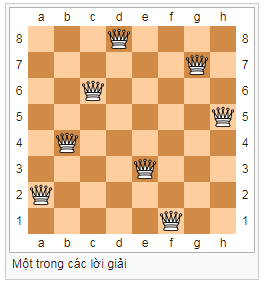
\includegraphics[scale=1]{image/hinhboard8x8}\\[1cm]
\end{center}

\subsubsection{Lịch sử}.
\\
Bài toán được đưa ra vào 1848 bởi kỳ thủ Max Bezzel, và sau đó nhiều nhà toán học, trong đó có Gauss và Georg Cantor, có các công trình về bài toán này và tổng quát nó thành bài toán xếp hậu. Các lời giải đầu tiên được đưa ra bởi Franz Nauck năm 1850. Nauck cũng đã tổng quát bài toán thành bài toán n quân hậu. Năm 1874, S. Gunther đưa ra phương pháp tìm lời giải bằng cách sử dụng định thức, và J.W.L. Glaisher hoàn chỉnh phương pháp này.

\subsubsection{Xây dựng một lời giải}.
\\
Có một giải thuật đơn giản tìm một lời giải cho bài toán n quân hậu với n = 1 hoặc n >= 4:\\
Chia n cho 12 lấy số dư r. (r= 8 với bài toán tám quân hậu).\\
Viết lần lượt các số chẵn từ 2 đến n.\\
Nếu số dư r là 3 hoặc 9, chuyển 2 xuống cuối danh sách.\\
Bổ sung lần lượt các số lẻ từ 1 đến n vào cuối danh sách, nhưng nếu r là 8, đổi chỗ từng cặp nghĩa là được 3, 1, 7, 5, 11, 9, ….\\
Nếu r = 2, đổi chỗ 1 và 3, sau đó chuyển 5 xuống cuối danh sách.\\
Nếu r = 3 hoặc 9, chuyển 1 và 3 xuống cuối danh sách.\\
Lấy danh sách trên làm danh sách chỉ số cột, ghép vào danh sách chỉ số dòng theo thứ tự tự nhiên ta được một lời giải của bài toán.\\
Sau đây là một số ví dụ: \\
$*$ 14 quân hậu (r = 2): 2, 4, 6, 8, 10, 12, 14, 3, 1, 7, 9, 11, 13, 5.\\
$*$ 15 quân hậu (r = 3): 4, 6, 8, 10, 12, 14, 2, 5, 7, 9, 11, 13, 15, 1, 3.\\
$*$ 20 quân hậu (r= 8): 2, 4, 6, 8, 10, 12, 14, 16, 18, 20, 3, 1, 7, 5, 11, 9, 15, 13, 19, 17.\\

\subsubsection{Số lời giải cho bài toán n quân hậu}.
\\
Ta có bảng sau đây cho n quân hậu
\begin{center}
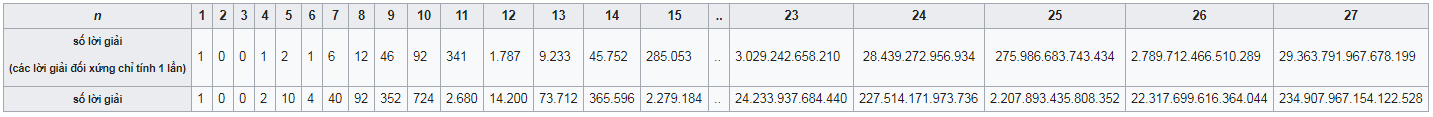
\includegraphics[scale=0.45]{image/n-board}\\[1cm]
\end{center}

\subsubsection{Giải thuật đệ quy và quay lui tìm kiếm tất cả các lời giải}.
\\
Trong giải thuật này, mỗi lời giải được ký hiệu bằng một mảng solution[1$..$n], trong đó solution[i]= j là cột mà quân hậu ở hàng thứ i đứng. Theo tính chất số học của các ô trên bàn cờ n x n, các ô trên các đường chéo cộng chứa ô (i, j) đều có tổng chỉ số hàng với chỉ số cột bằng i+j. Tổng này nhận các giá trị từ 2 đến 2n nên ta đánh số các đường chéo này từ 1 đến 2n-1. \\

Như vậy các ô trên đường chéo cộng thứ nhất có tổng chỉ số dòng và cột là 2, các ô trên đường chéo thứ k có tổng ấy là k+1. Ta dùng một mảng Boolean Ok\_plus[1..2n-1] để ký hiệu trạng thái đã có quân hậu nào trên đường chéo cộng thứ k chưa, nghĩa là Ok\_plus[k]=True nếu đã có một quân hậu đứng chiếm giữ đường chéo cộng thứ k.\\

Tương tự, các ô trên một đường chéo trừ có hiệu như nhau. Hiệu này nhận giá trị từ 1-n đến n- 1. Đánh số từ 1 đến 2n-1 từ đường chéo có hiệu chỉ số dòng trừ chỉ số cột là 1-n đến đường chéo có hiệu ấy bằng n-1. Khi đó đường chéo trừ thứ k có hiệu chỉ số dòng trừ chỉ số cột là k-n. Ta cũng dùng mảng ok\_minus[1..2n-1] để chỉ trạng thái của các đường chéo này.\\

Giải thuật này cố gắng đặt quân hậu ở dòng thứ i vào cột nào đó, bắt đầu từ dòng thứ nhất (luôn có thể đặt được). Nếu ở dòng thứ i ta đặt quân hậu vào cột thứ j, thì nó khống chế tất cả các ô trong cột thứ j, đường chéo cộng thứ i+j-1, đường chéo trừ thứ i-j+n. Nếu có thể đặt được quân hậu ở dòng i và i = n ta có một lời giải. Nếu đặt được và i < n ta tiếp tục cố gắng đặt quân hậu tiếp theo vào dòng thứ i+1. Nếu không đặt được, ta quay lại nhấc quân hậu ở dòng thứ i-1 và tìm phương án tiếp theo của dòng thứ i-1.



\subsection{Min-Conflict}

Mặc dù Trí tuệ nhân tạo và tối ưu hóa rời rạc đã biết đến và lý luận được về lập trình ràng buộc (CSP - Constraint Satisfaction Problems), nhưng mãi tới năm 1990, các bài toán CSP mới được giải bằng các thuật toán. Ban đầu, Mark Johnson thuộc viện Space Telescope Science đã tìm kiếm một phương pháp để lên lịch các quan sát thiên văn trên kính viễn vọng không gian Hubble. Với người đồng nghiệp Hans-Martin Adorf của Cơ quan Điều phối Châu Âu về kính viễn vọng Không gian, ông đã tạo ra một mạng lưới thần kinh có khả năng giải quyết vấn đề bài toán N-con hậu (Cho 1024 con hậu). Steven Minton và Andy Philips đã phân tích thuật toán mạn nowrron và tách nó thành hai giai đoạn (1) một phép gán ban đầu sử dụng thuật toán tham lam (2) Các pha giảm thiểu xung đột (Sau này được gọi là "Xung đột tối thiểu").  Kết quả nghiên cứu này được công bố trong bài báo AAAI-90, Philip Larird đã phân tích luận lý toán học của thuật toán.

\subsubsection{Min-Conflict Hill Climbing algorithm}.\\
{\bfseries Mã giả của thuật toán}\\
procedure GenerateLocalMoves(s, TotalMoves) \\
begin \\
    \hspace{1cm}  M' $\gets$  ø, BestCost $\gets$ f(s) \\
    \hspace{1cm} choose randomly a variable v in conflict \\ 
    \hspace{1cm} choose a value d for v (d $\neq$ dcurr) that minimizes the number of conflicts for v. \\
   \hspace{1cm}  m $\gets$ {v, d} \\ 
    \hspace{1cm} if f(s $\oplus$ m) $\leq$ BestCost then  // accepts improving moves and sideways moves \\
          \hspace{2cm} begin \\
            \hspace{2cm}  if f(s $\oplus$ m) < BestCost then \\
            \hspace{2cm}  begin \\
                  \hspace{3cm}BestCost $\gets$ f(s $\oplus$ m); M’ $\gets$ ø\\
            \hspace{2cm}  end \\
              M $\gets$  M’ ø {m} \\
           \hspace{2cm} end \\
     \hspace{1cm} if M' = ø then TotalMoves $\gets$ MaxMoves\\
    \hspace{1cm} return M’\\
end\\

\subsubsection{Min-Conflict Random Walk algorithm}.\\
{\bfseries Mã giả của thuật toán}\\
begin\\
   generate randomly an initial solution s\\
   n\_iter := 0; n\_moves := 0\\
   while f(s) > max\_cost and n\_moves < max\_moves do\\
      if p > random number between 0 and 1 then\\
        choose randomly a variable V in conflict\\
        choose randomly a value v’ for V\\
      else\\
         choose randomly a variable V in conflict\\
         choose a value v’ for V that minimizes the number of conflicts for V.\\
         (the current value is chosen only if all the other values increase the number of \\
           violated constraints.)\\
       if v’ is different from the current value of V then\\
          assign v’ to V\\
          n\_moves := n\_moves + 1\\
       n\_iter := n\_iter + 1\\
    endwhile\\
    output(s)\\
end\\
%%%%%%%%%%%%%%
\section{Kết Luận }\label{result}
Tài liệu được thực hiện  với sự giúp đỡ tận tình của giáo viên hướng dẫn, Thầy TS. Dương Tuấn Anh\\
Trong quá trình nghiên cứu, thực hiện không thể tránh khỏi những  thiếu sót, kính mong quý thầy  cô và các bạn đóng góp thêm để tài liệu thêm hoàn thiện.\\
Xin chân thành cảm ơn.




%%%%%%%%%%%%%%
\section{Tài liệu Tham Khảo }




%%%%%%%%%%%%%%%%%%%%%%%%%%%%%%%%%

http://en.wikipedia.org\\
http://globaledu.com.vn/Thong-Tin-Chi-Tiet/1881/1881\\
http://library.williams.edu/citing/styles/acs.php\\

%%%%%%%%%%%%%%

\end{document}



